\newpage
\section{Complete Data Set for Compression Analysis \label{Appendix: Complete Data Set for Compression Analysis}}

For full comparison given below are the full data sets for the compression analysis.

\begin{figure}[H]
\centering

    \begin{subfigure}{0.32\textwidth}
        \centering
        \caption{\label{fig: All-Hemisphere-ContourPlot-1}}
        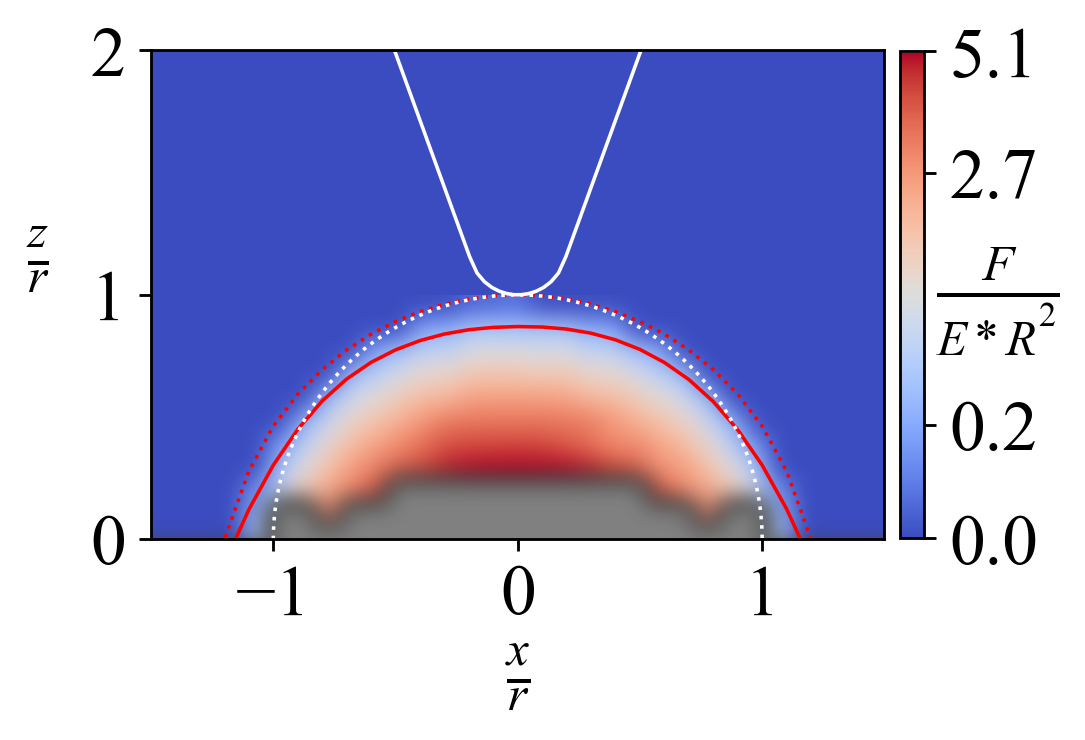
\includegraphics[width=1\linewidth]{Figures/Hemisphere-ContourPlot-1.png}
    \end{subfigure}
    \hfill     
    \begin{subfigure}{0.32\textwidth}
        \centering
        \caption{\label{fig: All-Hemisphere-ContourPlotNI-1}}
        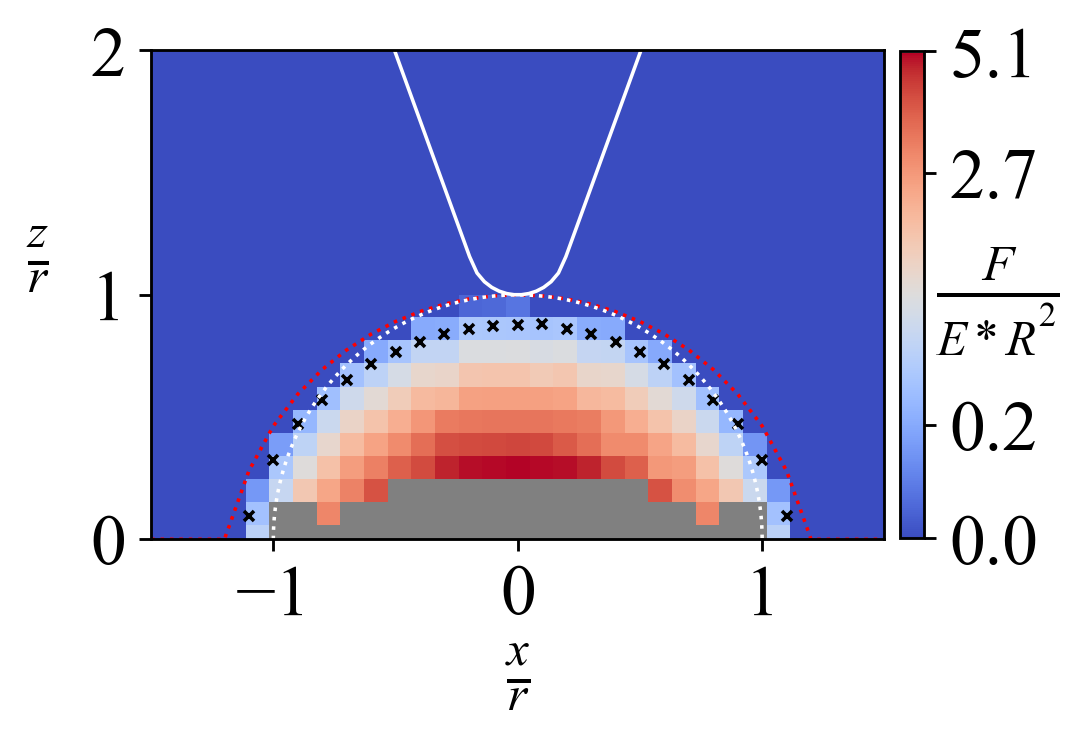
\includegraphics[width=1\linewidth]{Figures/Hemisphere-ContourPlotNI-1.png}
    \end{subfigure}
    \hfill     
    \begin{subfigure}{0.32\textwidth}
        \centering
        \caption{\label{fig: All-Hemisphere-LineContour-1}}
        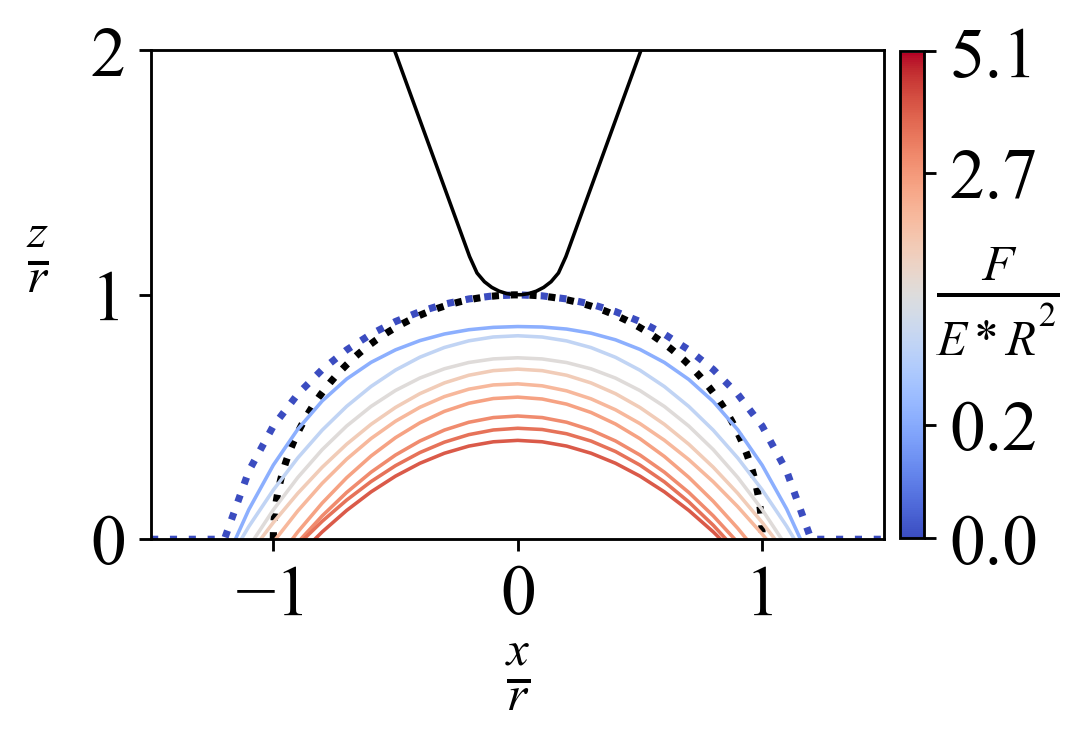
\includegraphics[width=1\linewidth]{Figures/Hemisphere-LineContour-1.png}
    \end{subfigure}
    % \hfill  
    % \begin{subfigure}{0.32\textwidth}
    %     \centering
    %     \caption{\label{fig: All-Hemisphere-FInterpolate-1}}
    %     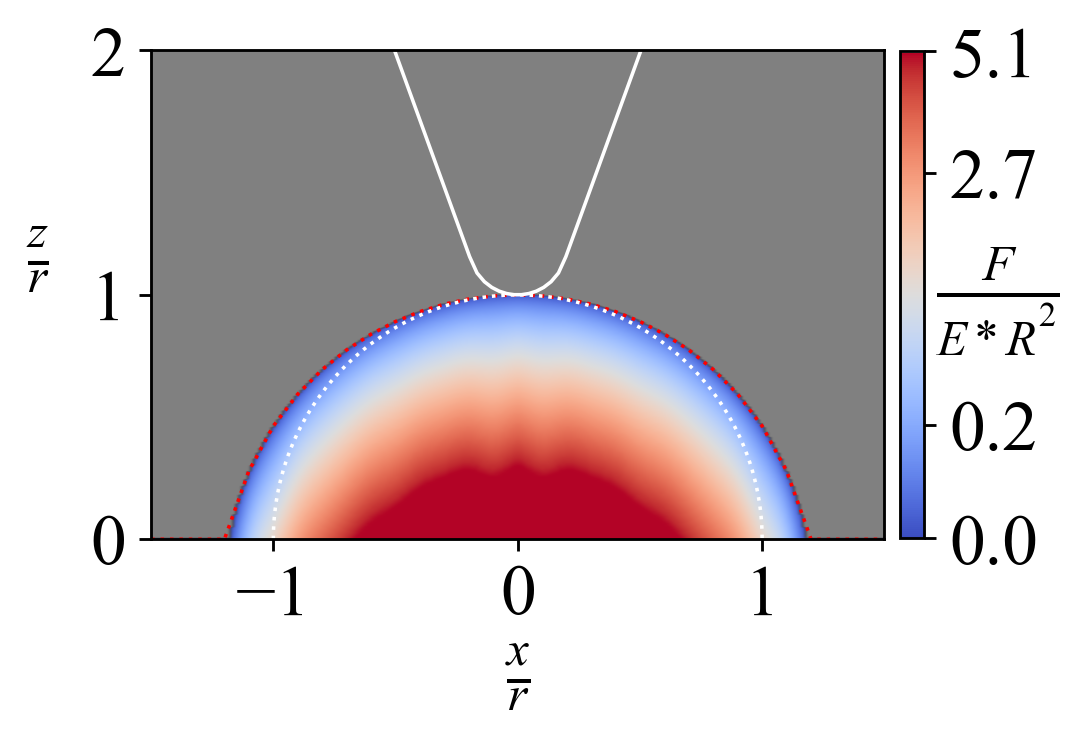
\includegraphics[width=1\linewidth]{Figures/Hemisphere-FInterpolate-1.png}
    % \end{subfigure}   



    \hfill
    \vspace{-0.3in}


    
    \begin{subfigure}{0.32\textwidth}
        \centering
        \caption{\label{fig: All-Hemisphere-ContourPlot-3}}
        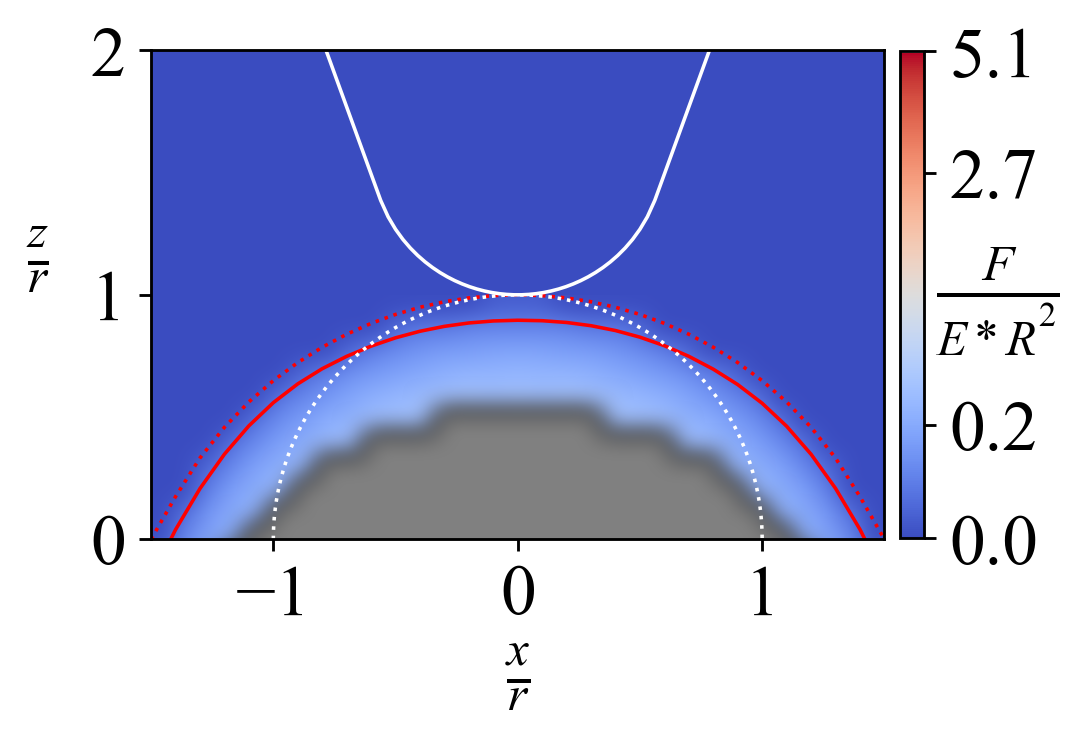
\includegraphics[width=1\linewidth]{Figures/Hemisphere-ContourPlot-3.png}
    \end{subfigure}
    \hfill
    \begin{subfigure}{0.32\textwidth}
        \centering
        \caption{\label{fig: All-Hemisphere-ContourPlotNI-3}}
        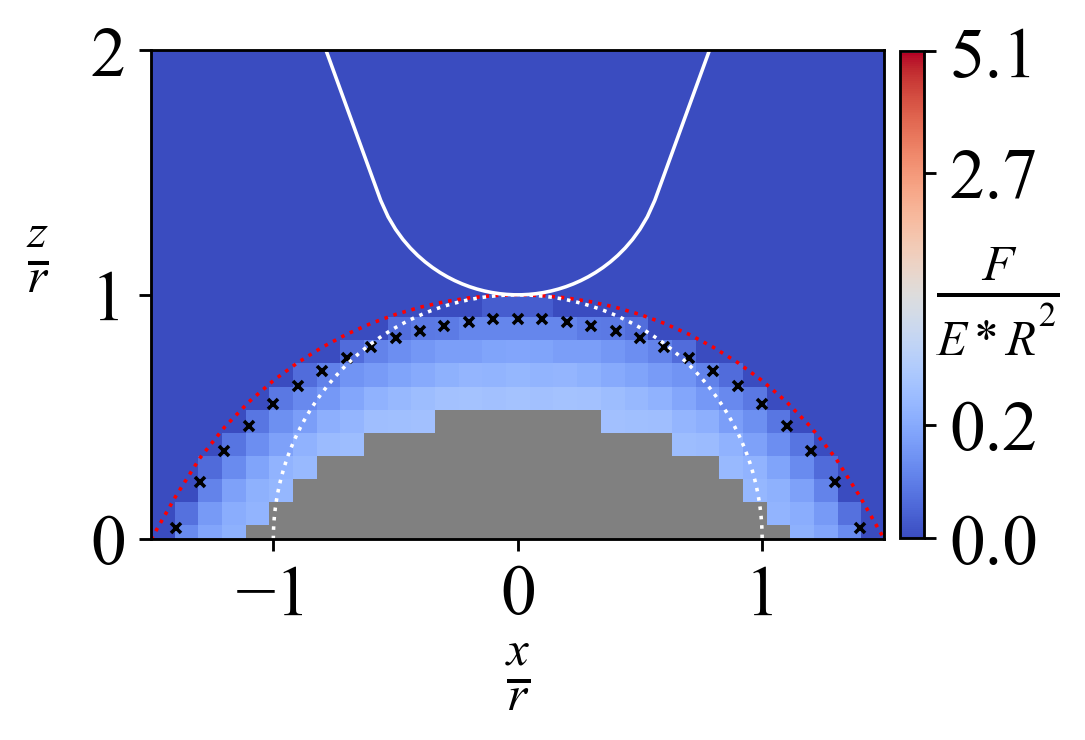
\includegraphics[width=1\linewidth]{Figures/Hemisphere-ContourPlotNI-3.png}
    \end{subfigure}
    \hfill
    \begin{subfigure}{0.32\textwidth}
        \centering
        \caption{\label{fig: All-Hemisphere-LineContour-3}}
        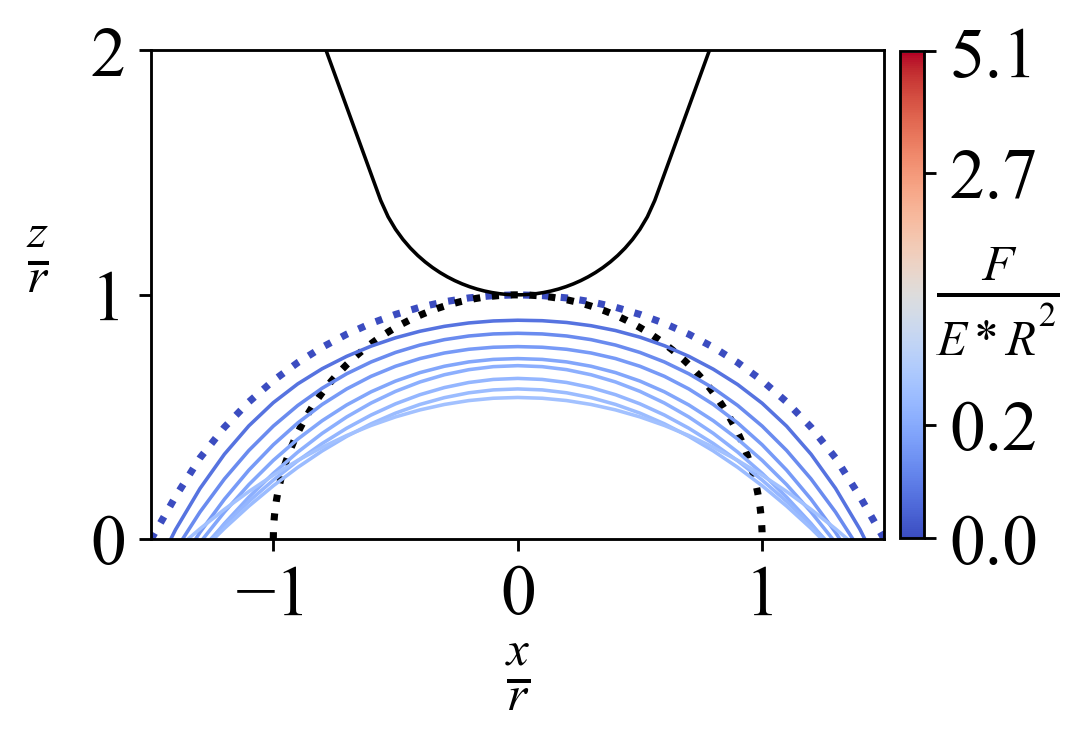
\includegraphics[width=1\linewidth]{Figures/Hemisphere-LineContour-3.png}
    \end{subfigure}
    % \hfill 
    % \begin{subfigure}{0.32\textwidth}
    %     \centering
    %     \caption{\label{fig: All-Hemisphere-FInterpolate-3}}
    %     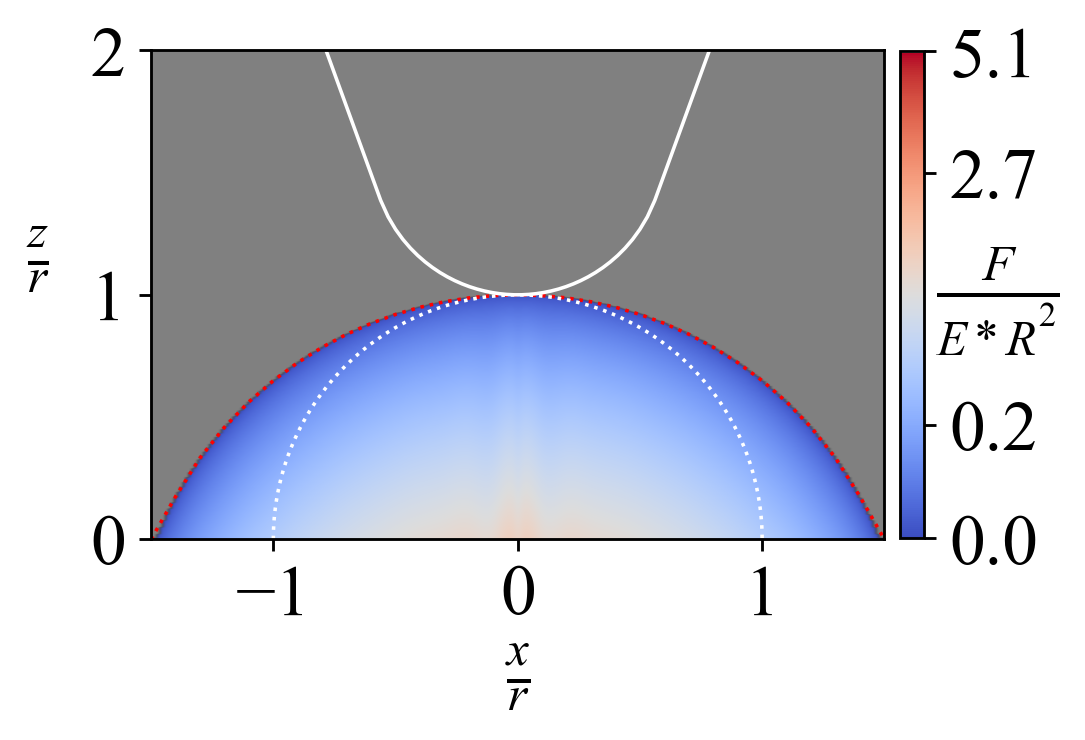
\includegraphics[width=1\linewidth]{Figures/Hemisphere-FInterpolate-3.png}
    % \end{subfigure}



    \hfill
    \vspace{-0.3in}


    
    \begin{subfigure}{0.32\textwidth}
        \centering
        \caption{\label{fig: All-Hemisphere-ContourPlot-5}}
        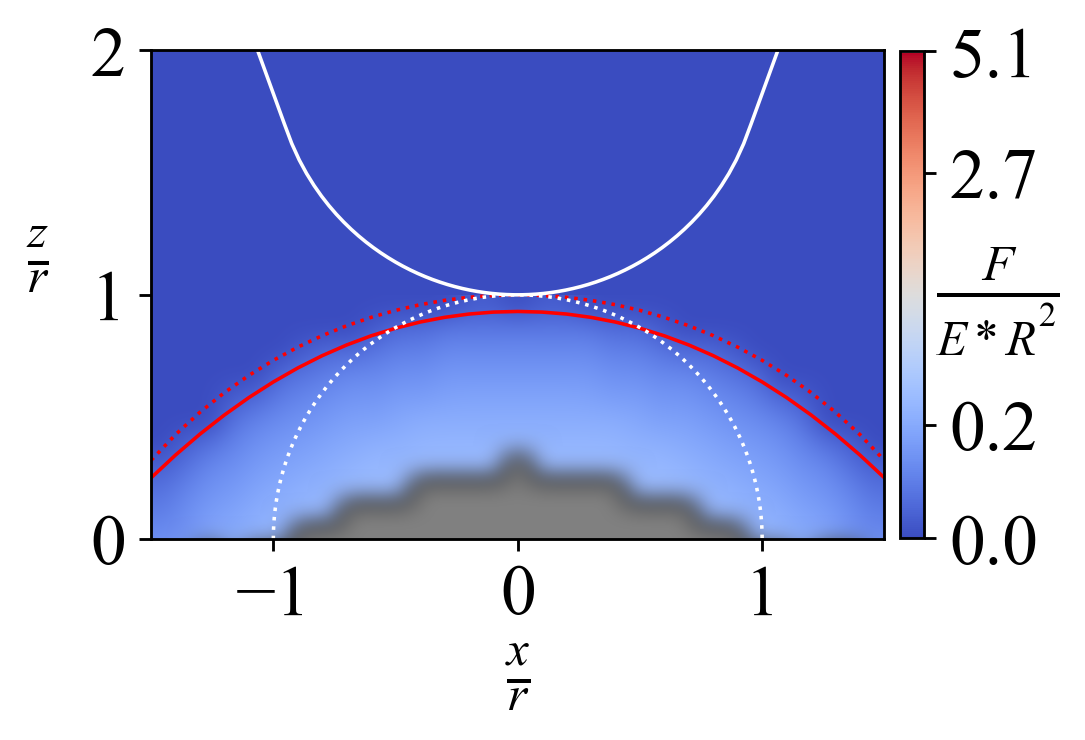
\includegraphics[width=1\linewidth]{Figures/Hemisphere-ContourPlot-5.png}
    \end{subfigure}   
    \hfill
   \begin{subfigure}{0.32\textwidth}
        \centering
        \caption{\label{fig: All-Hemisphere-ContourPlotNI-5}}
        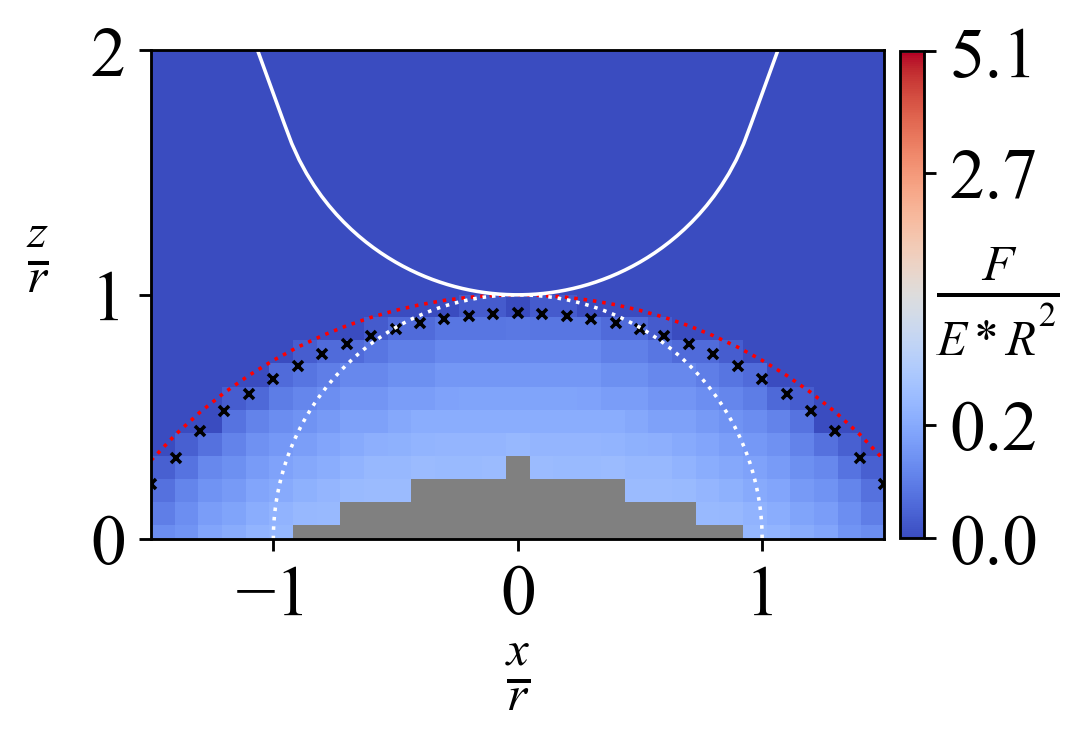
\includegraphics[width=1\linewidth]{Figures/Hemisphere-ContourPlotNI-5.png}
    \end{subfigure}   
    \hfill    
    \begin{subfigure}{0.32\textwidth}
        \centering
        \caption{\label{fig: All-Hemisphere-LineContour-5}}
        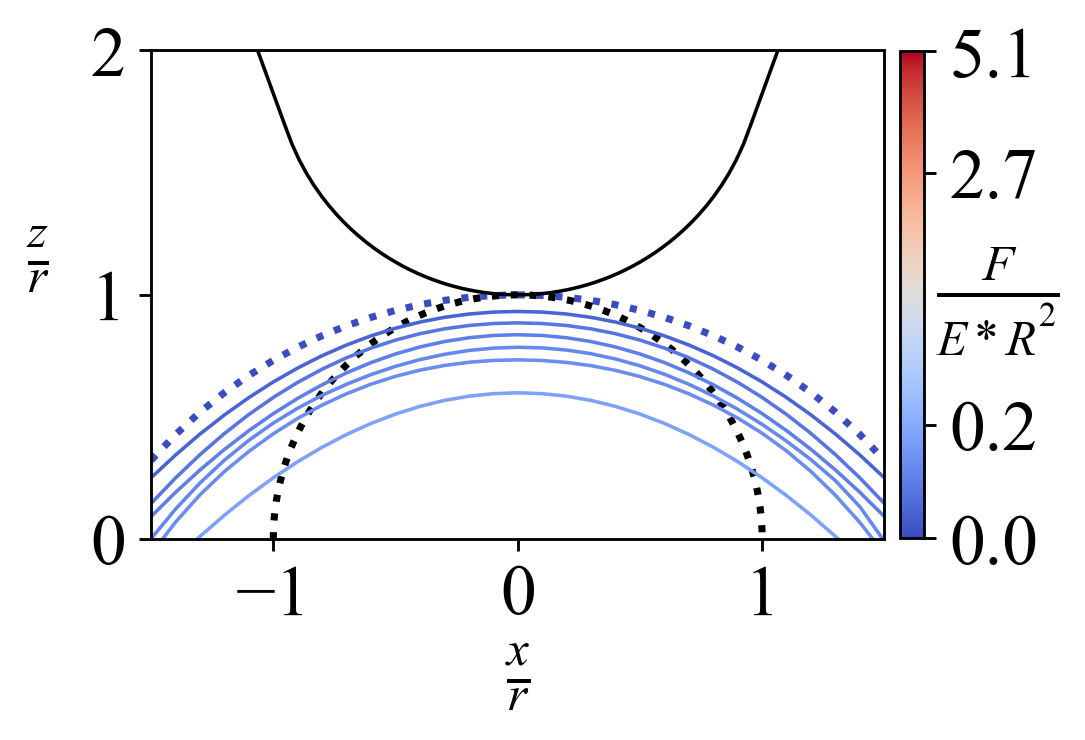
\includegraphics[width=1\linewidth]{Figures/Hemisphere-LineContour-5.png}
    \end{subfigure}   
    % \hfill
    % \begin{subfigure}{0.32\textwidth}
    %     \centering
    %     \caption{\label{fig: All-Hemisphere-FInterpolate-5}}
    %     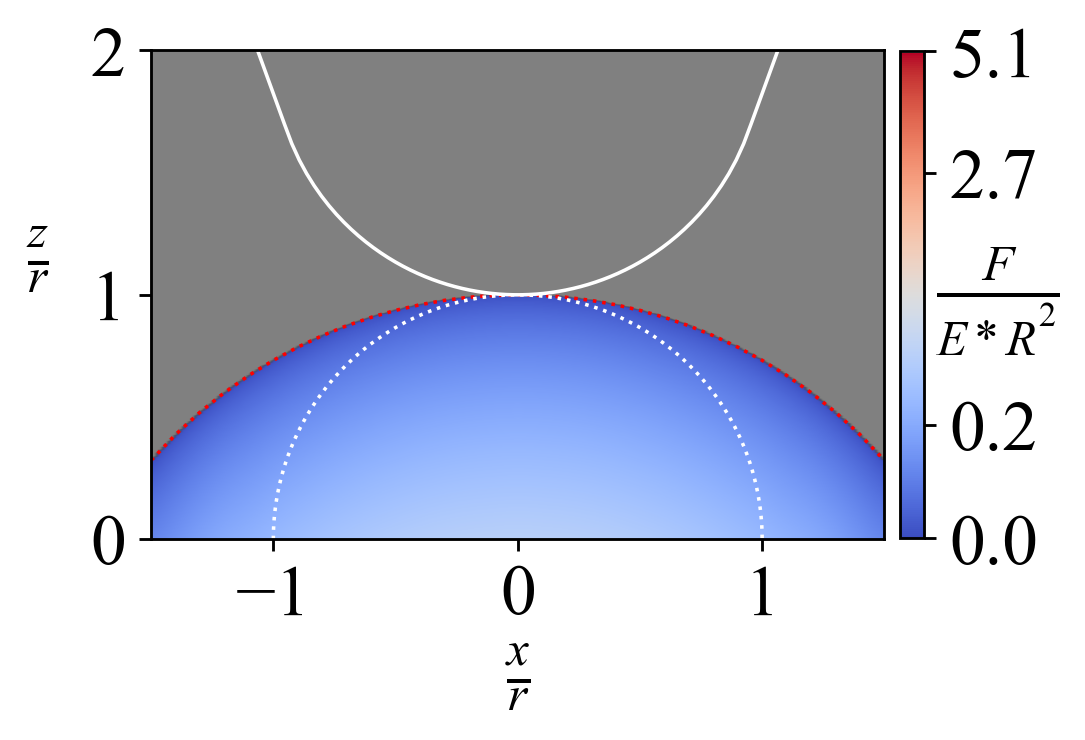
\includegraphics[width=1\linewidth]{Figures/Hemisphere-FInterpolate-5.png}
    % \end{subfigure}   



    \hfill
    \vspace{-0.3in}
    
    
    
    \begin{subfigure}{0.32\textwidth}
        \centering
        \caption{\label{fig: All-Hemisphere-ContourPlot-7}}
        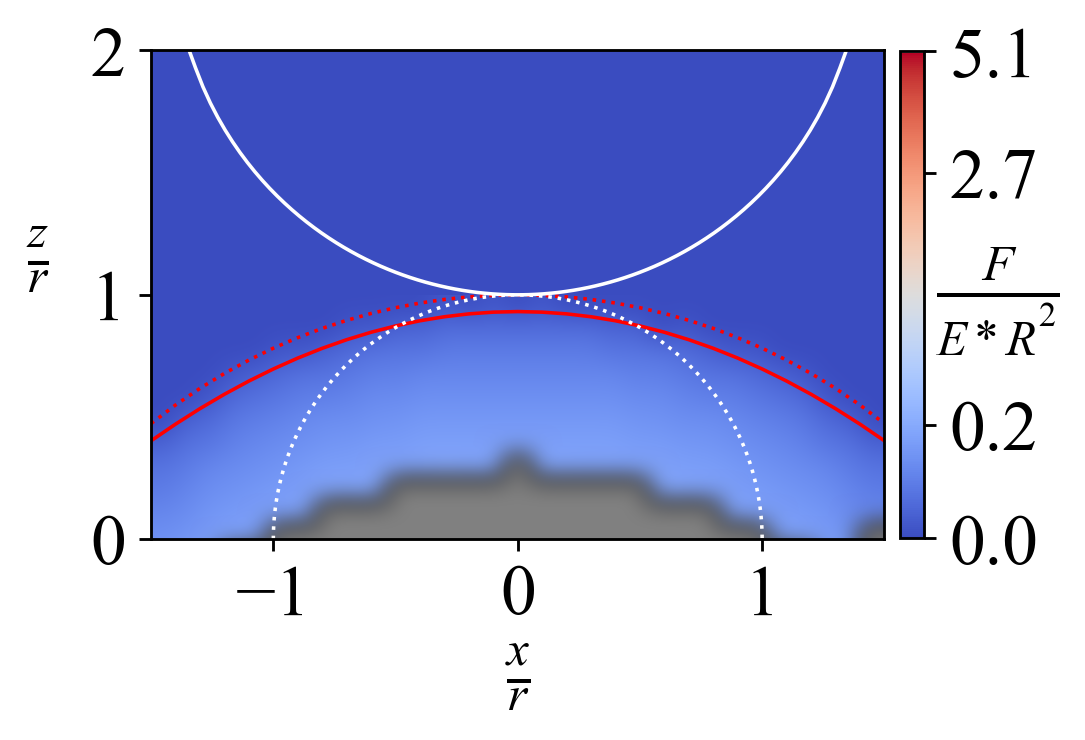
\includegraphics[width=1\linewidth]{Figures/Hemisphere-ContourPlot-7.png}
    \end{subfigure}  
    \hfill  
    \begin{subfigure}{0.32\textwidth}
        \centering
        \caption{\label{fig: All-Hemisphere-ContourPlotNI-7}}
        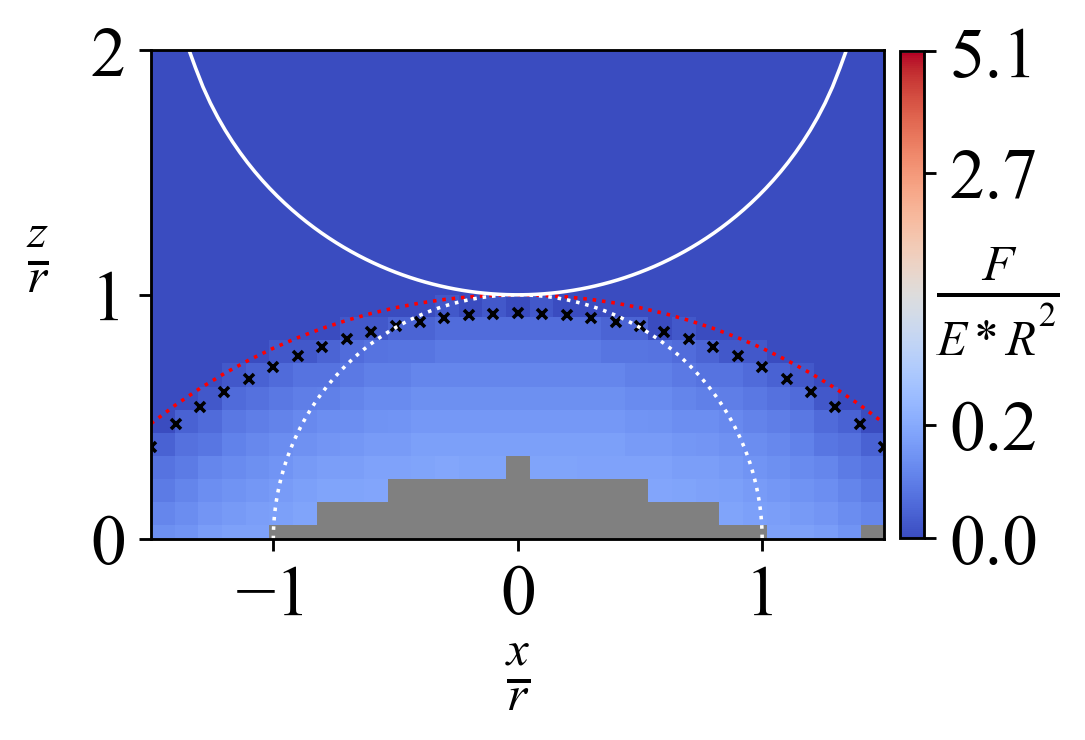
\includegraphics[width=1\linewidth]{Figures/Hemisphere-ContourPlotNI-7.png}
    \end{subfigure}  
    \hfill  
    \begin{subfigure}{0.32\textwidth}
        \centering
        \caption{\label{fig: All-Hemisphere-LineContour-7}}
        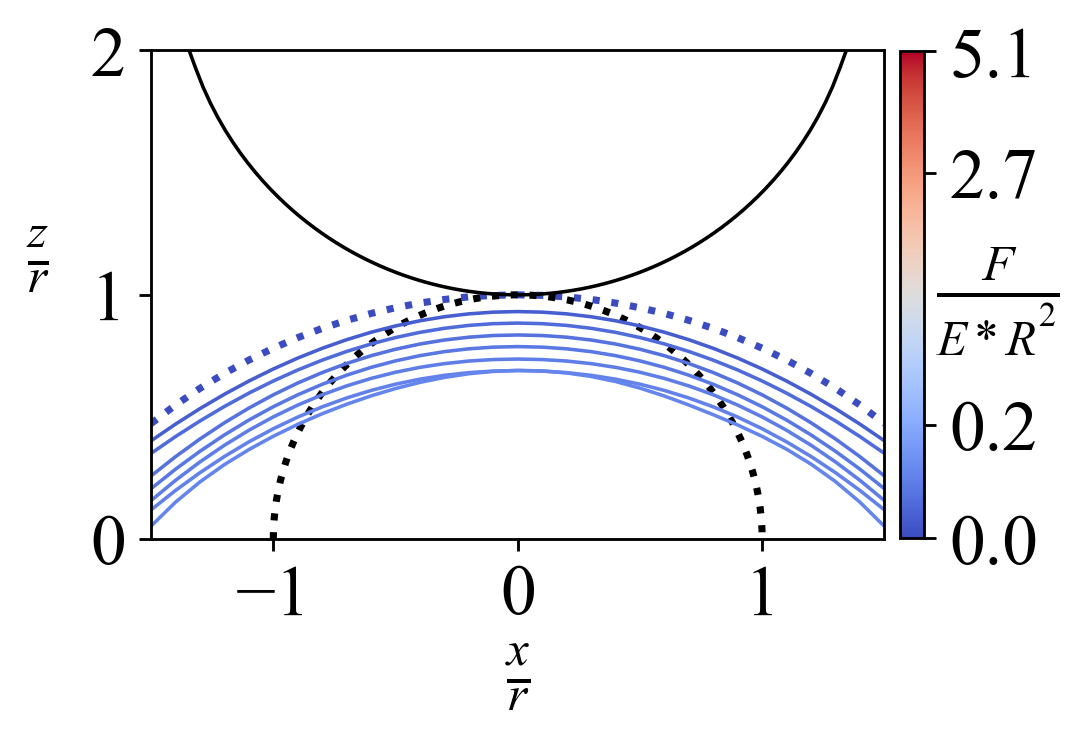
\includegraphics[width=1\linewidth]{Figures/Hemisphere-LineContour-7.png}
    \end{subfigure}  
    % \hfill  
    % \begin{subfigure}{0.32\textwidth}
    %     \centering
    %     \caption{\label{fig: All-Hemisphere-FInterpolate-7}}
    %     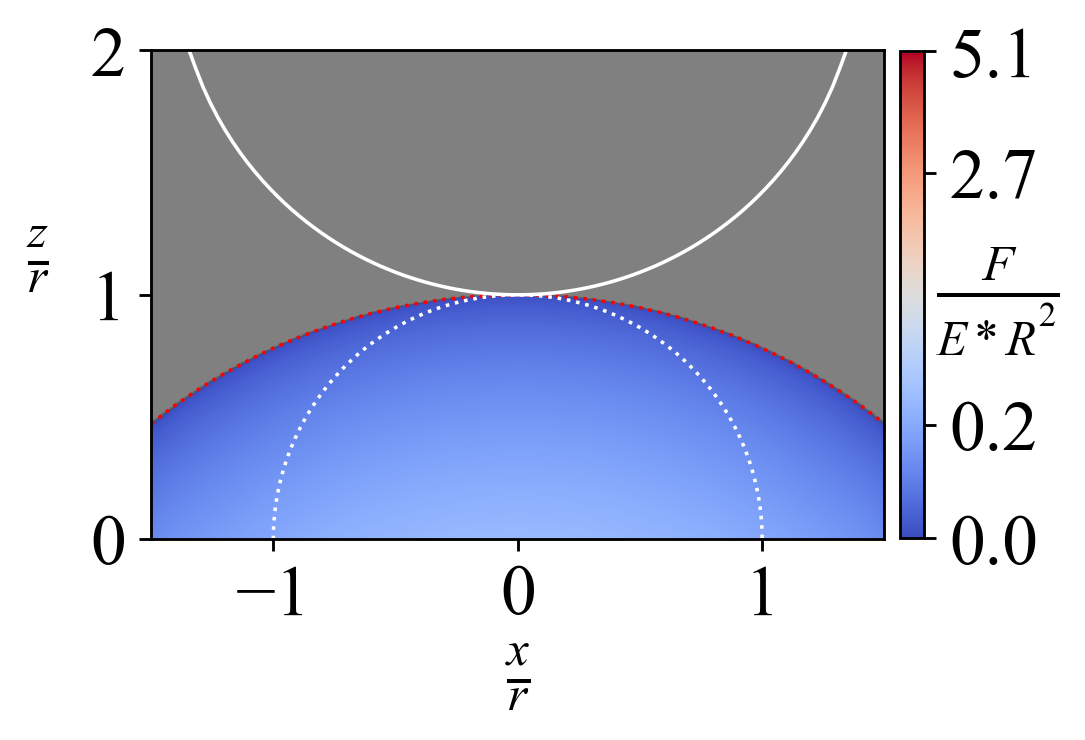
\includegraphics[width=1\linewidth]{Figures/Hemisphere-FInterpolate-7.png}
    % \end{subfigure}  


    
    \hfill
    \vspace{-0.3in}
    

    
    \begin{subfigure}{0.32\textwidth}
        \centering
        \caption{\label{fig: All-Hemisphere-ContourPlot-9}}
        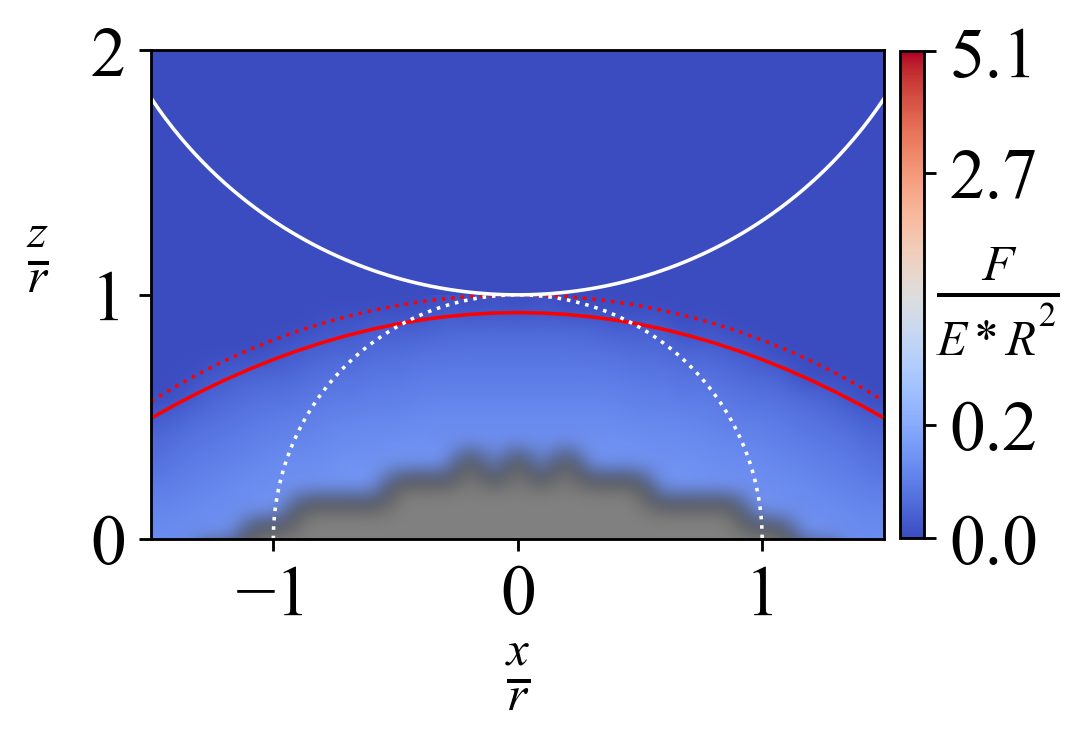
\includegraphics[width=1\linewidth]{Figures/Hemisphere-ContourPlot-9.png}
    \end{subfigure}  
    \hfill
        \begin{subfigure}{0.32\textwidth}
        \centering
        \caption{\label{fig: All-Hemisphere-ContourPlotNI-9}}
        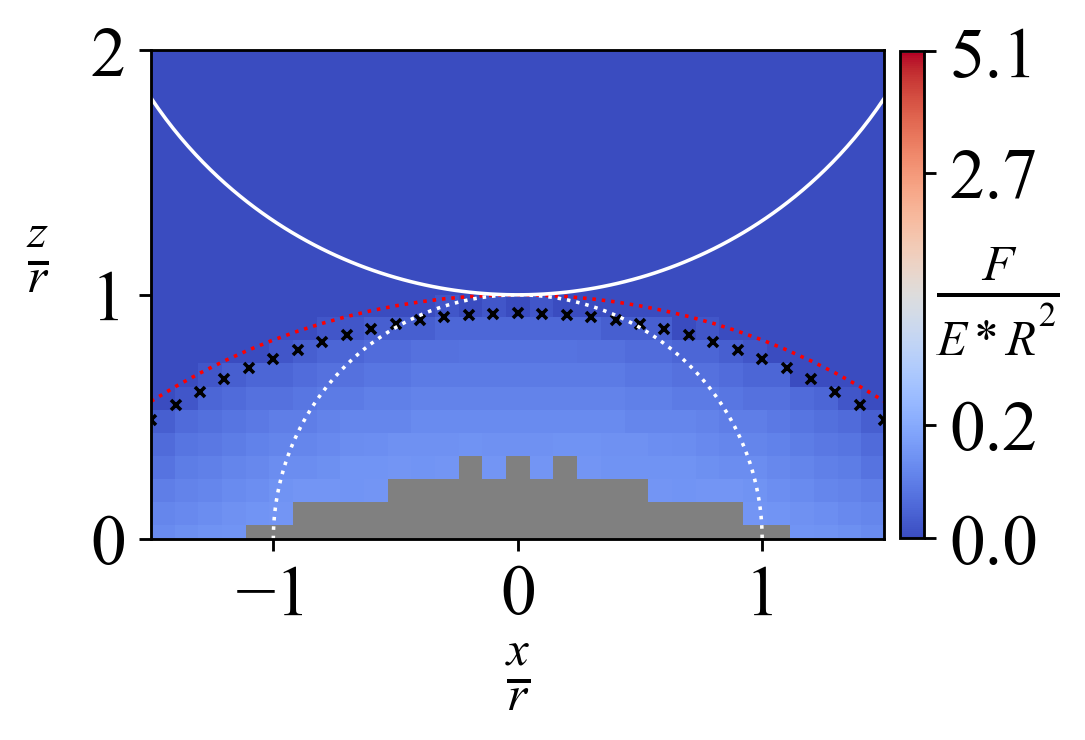
\includegraphics[width=1\linewidth]{Figures/Hemisphere-ContourPlotNI-9.png}
    \end{subfigure}
    \hfill
    \begin{subfigure}{0.32\textwidth}
        \centering
        \caption{\label{fig: All-Hemisphere-LineContour-9}}
        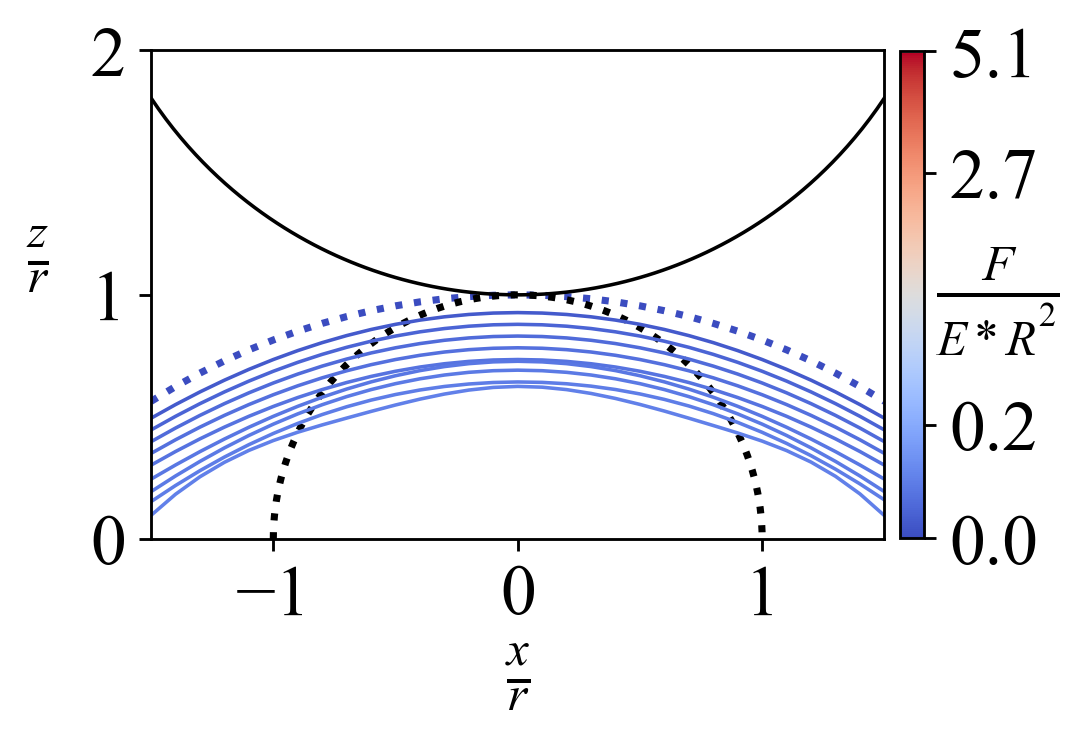
\includegraphics[width=1\linewidth]{Figures/Hemisphere-LineContour-9.png}
    \end{subfigure} 
    % \hfill
    % \begin{subfigure}{0.32\textwidth}
    %     \centering
    %     \caption{\label{fig: All-Hemisphere-FInterpolate-9}}
    %     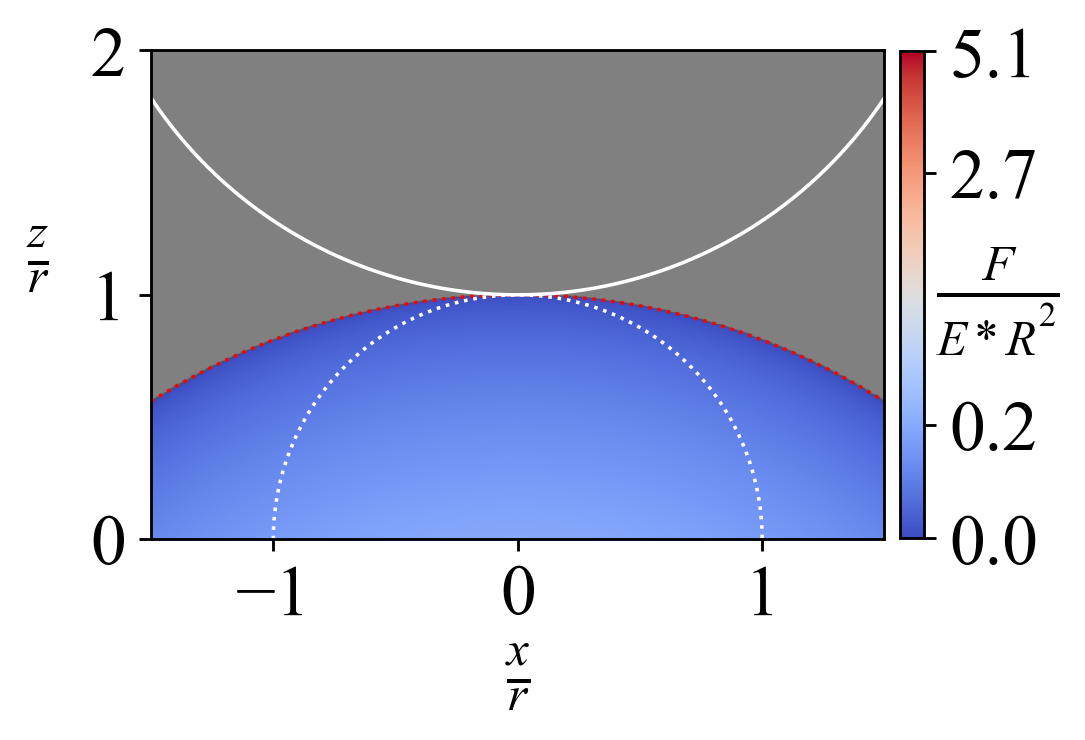
\includegraphics[width=1\linewidth]{Figures/Hemisphere-FInterpolate-9.png}
    % \end{subfigure}  
    
    \vspace{-0.1in}
    
    \caption{\label{fig: All-Hemisphere-ContourPlot} }
\end{figure}









\begin{figure}[H]
\centering

    \begin{subfigure}{0.32\textwidth}
        \centering
        \caption{\label{fig: All-Wave-ContourPlot-1}}
        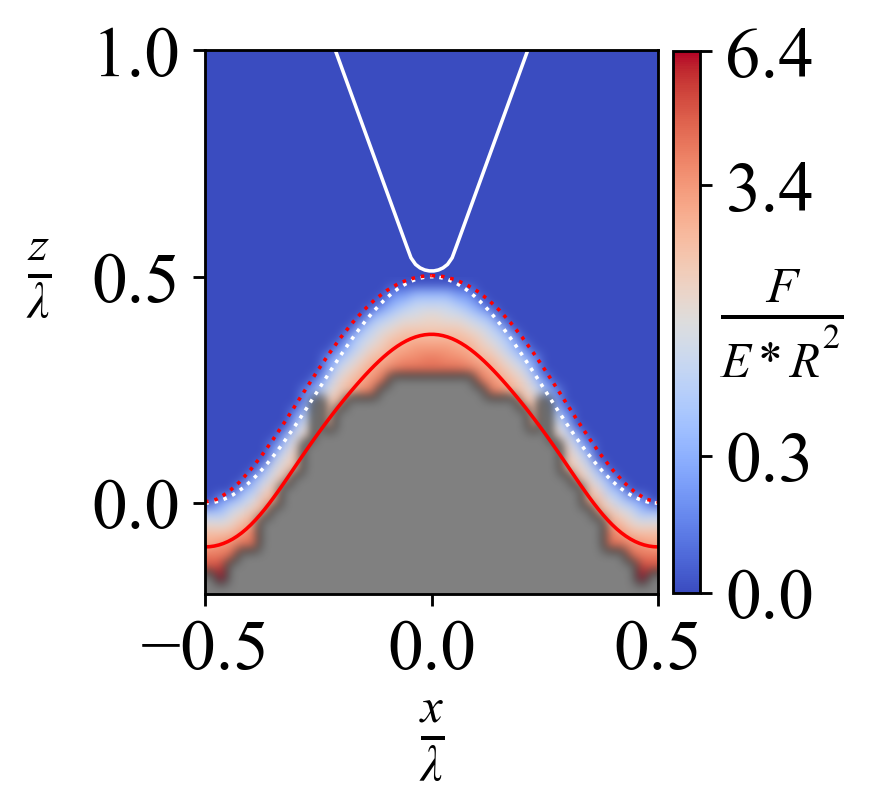
\includegraphics[width=1\linewidth]{Figures/Wave-ContourPlot-1.png}
    \end{subfigure}
    \hfill     
    \begin{subfigure}{0.32\textwidth}
        \centering
        \caption{\label{fig: All-Wave-ContourPlotNI-1}}
        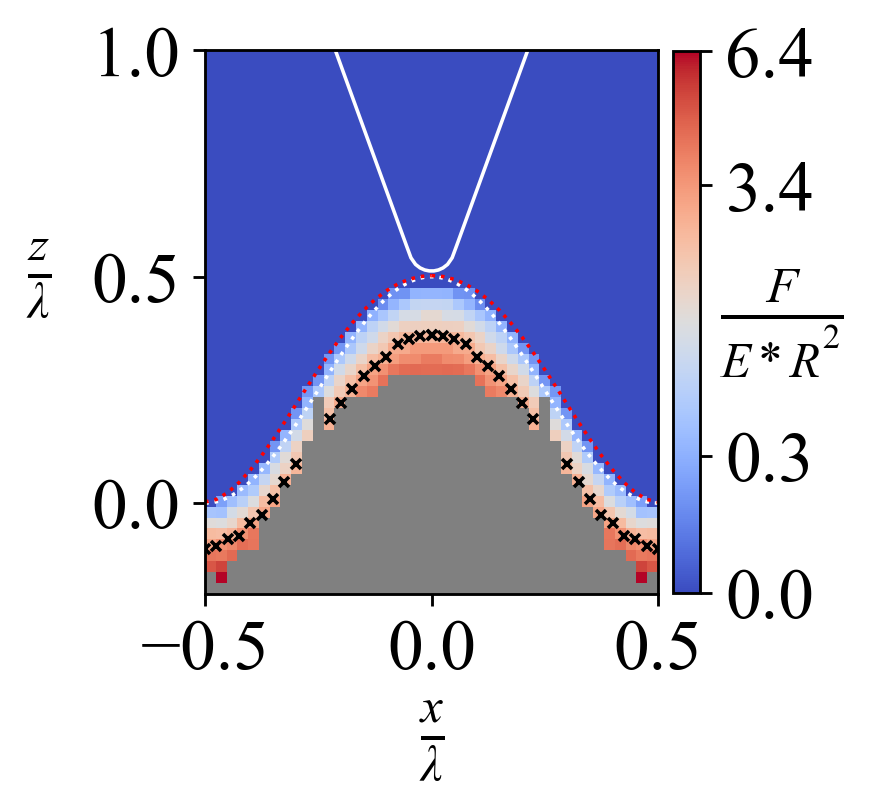
\includegraphics[width=1\linewidth]{Figures/Wave-ContourPlotNI-1.png}
    \end{subfigure}
    \hfill     
    \begin{subfigure}{0.32\textwidth}
        \centering
        \caption{\label{fig: All-Wave-LineContour-1}}
        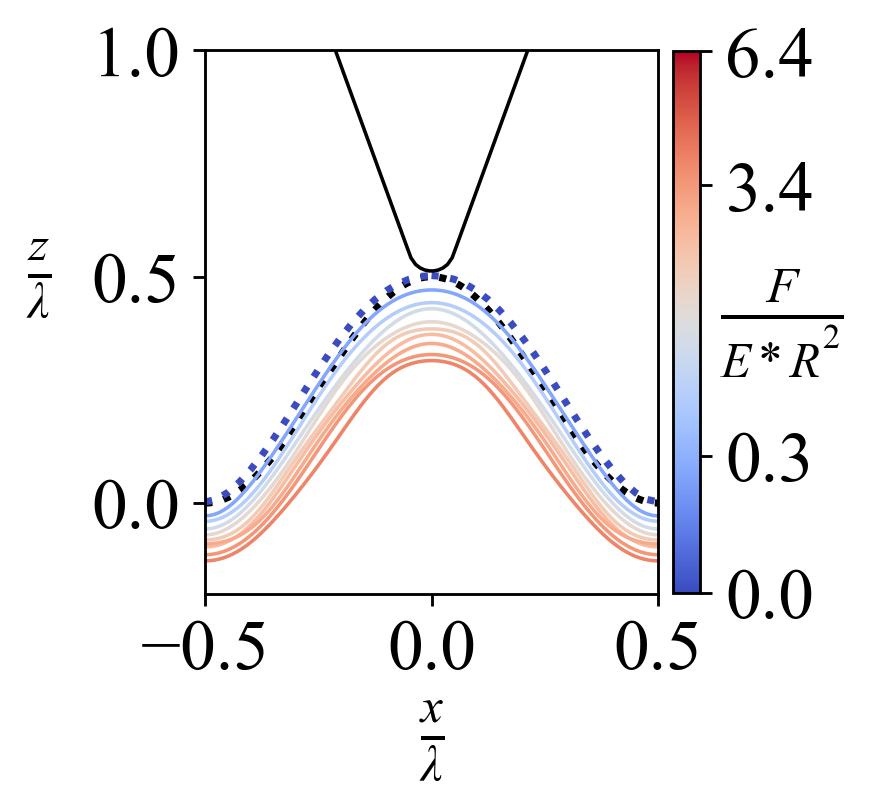
\includegraphics[width=1\linewidth]{Figures/Wave-LineContour-1.png}
    \end{subfigure}
    % \hfill  
    % \begin{subfigure}{0.32\textwidth}
    %     \centering
    %     \caption{\label{fig: All-Wave-FInterpolate-1}}
    %     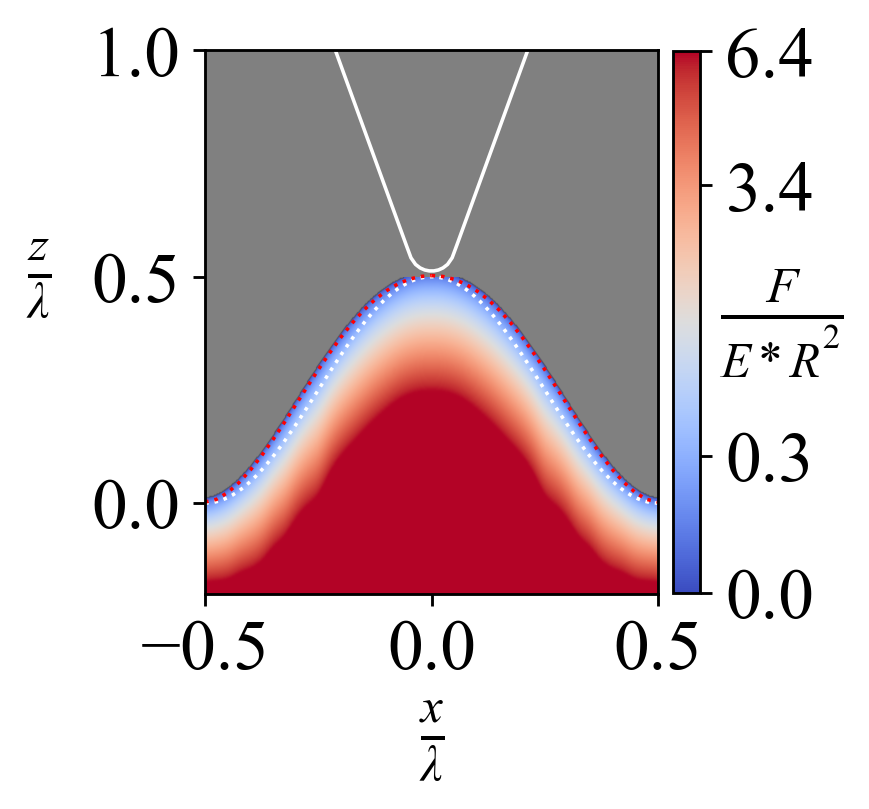
\includegraphics[width=1\linewidth]{Figures/Wave-FInterpolate-1.png}
    % \end{subfigure}   



    \hfill
    \vspace{-0.3in}


    
    \begin{subfigure}{0.32\textwidth}
        \centering
        \caption{\label{fig: All-Wave-ContourPlot-3}}
        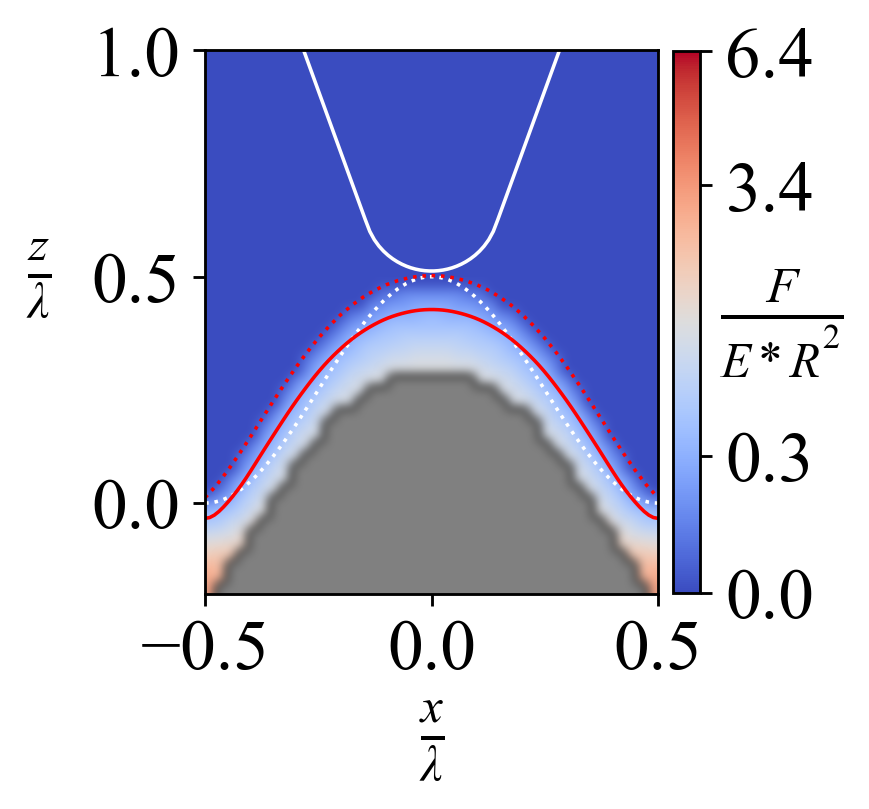
\includegraphics[width=1\linewidth]{Figures/Wave-ContourPlot-3.png}
    \end{subfigure}
    \hfill
    \begin{subfigure}{0.32\textwidth}
        \centering
        \caption{\label{fig: All-Wave-ContourPlotNI-3}}
        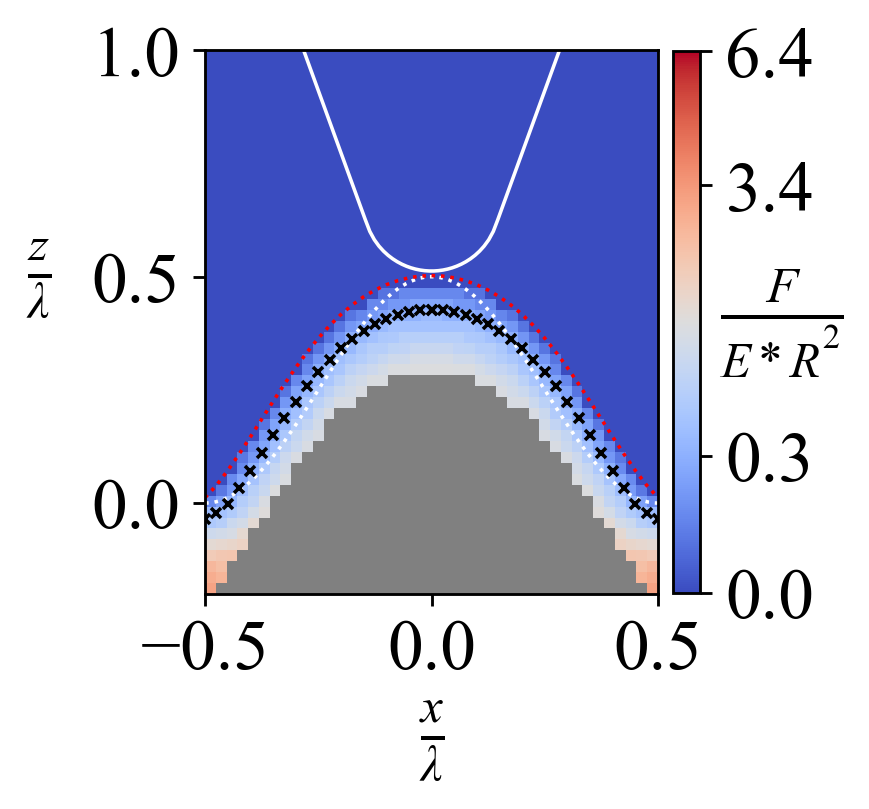
\includegraphics[width=1\linewidth]{Figures/Wave-ContourPlotNI-3.png}
    \end{subfigure}
    \hfill
    \begin{subfigure}{0.32\textwidth}
        \centering
        \caption{\label{fig: All-Wave-LineContour-3}}
        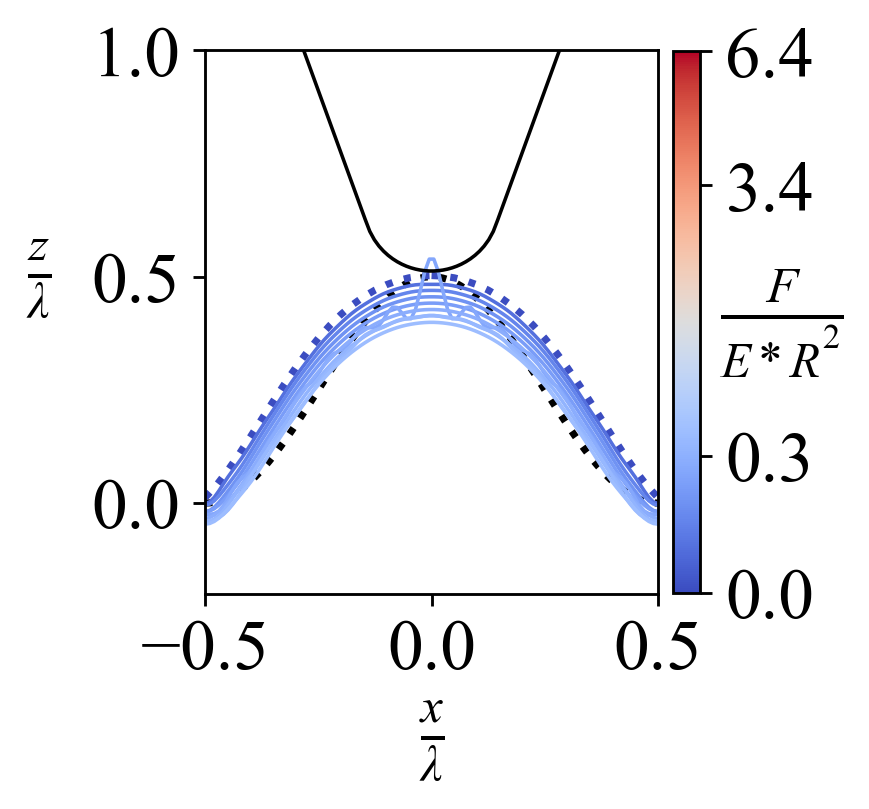
\includegraphics[width=1\linewidth]{Figures/Wave-LineContour-3.png}
    \end{subfigure}
    % \hfill 
    % \begin{subfigure}{0.32\textwidth}
    %     \centering
    %     \caption{\label{fig: All-Wave-FInterpolate-3}}
    %     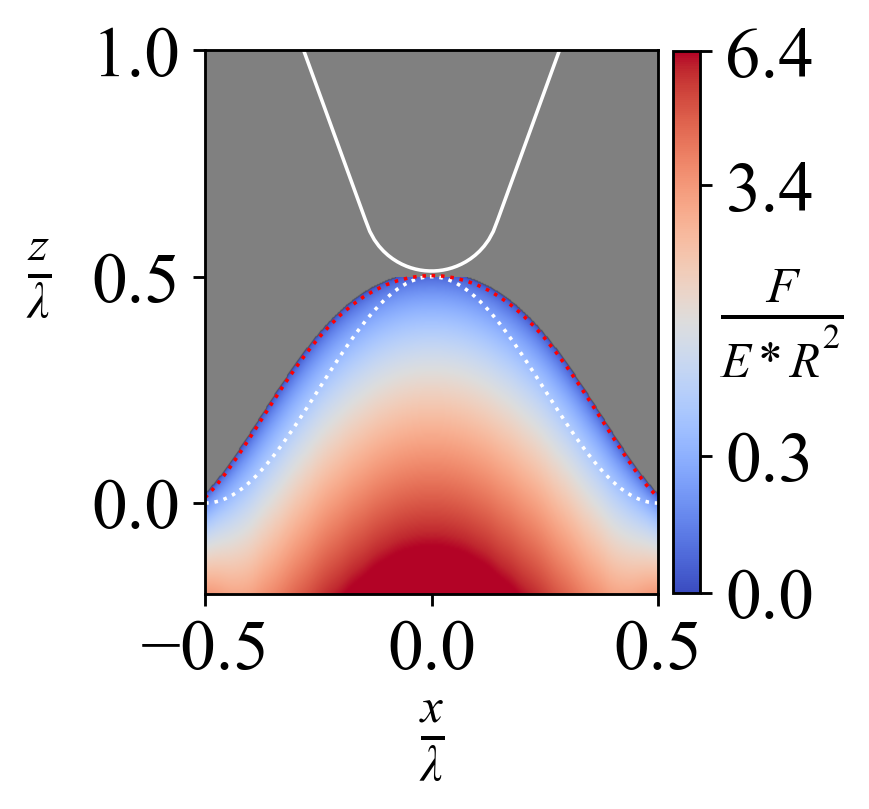
\includegraphics[width=1\linewidth]{Figures/Wave-FInterpolate-3.png}
    % \end{subfigure}



    \hfill
    \vspace{-0.3in}


    
    \begin{subfigure}{0.32\textwidth}
        \centering
        \caption{\label{fig: All-Wave-ContourPlot-5}}
        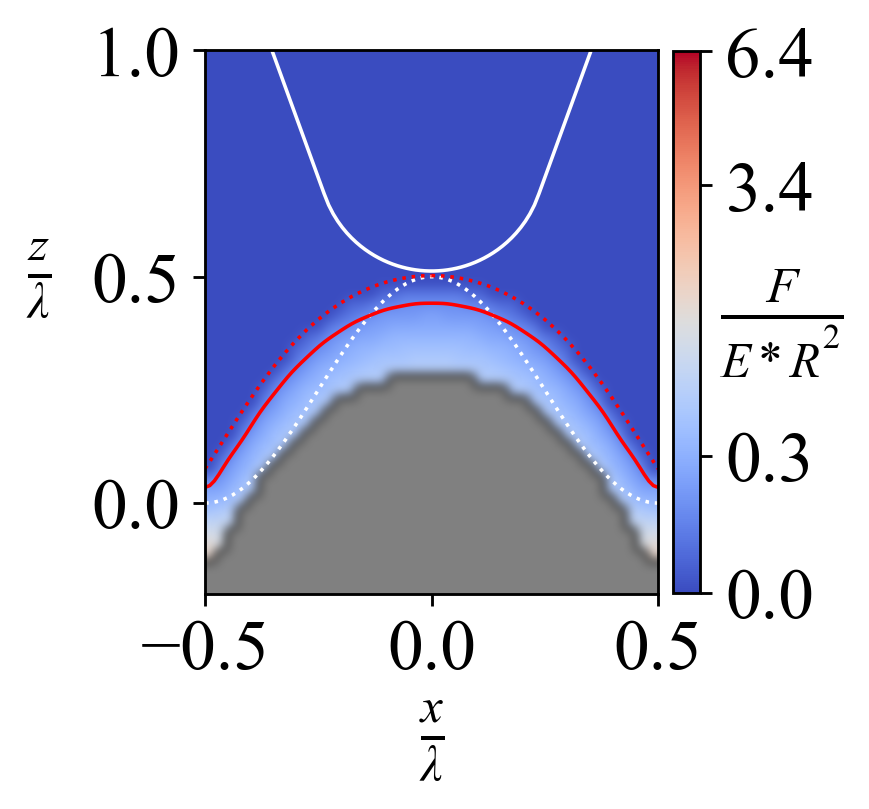
\includegraphics[width=1\linewidth]{Figures/Wave-ContourPlot-5.png}
    \end{subfigure}   
    \hfill
   \begin{subfigure}{0.32\textwidth}
        \centering
        \caption{\label{fig: All-Wave-ContourPlotNI-5}}
        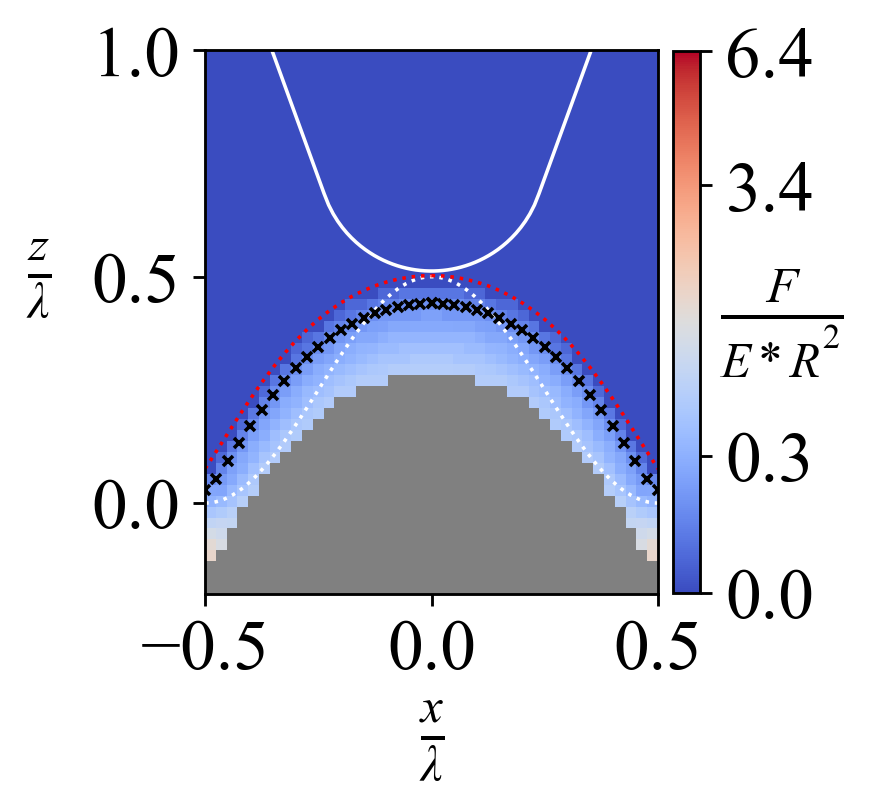
\includegraphics[width=1\linewidth]{Figures/Wave-ContourPlotNI-5.png}
    \end{subfigure}   
    \hfill    
    \begin{subfigure}{0.32\textwidth}
        \centering
        \caption{\label{fig: All-Wave-LineContour-5}}
        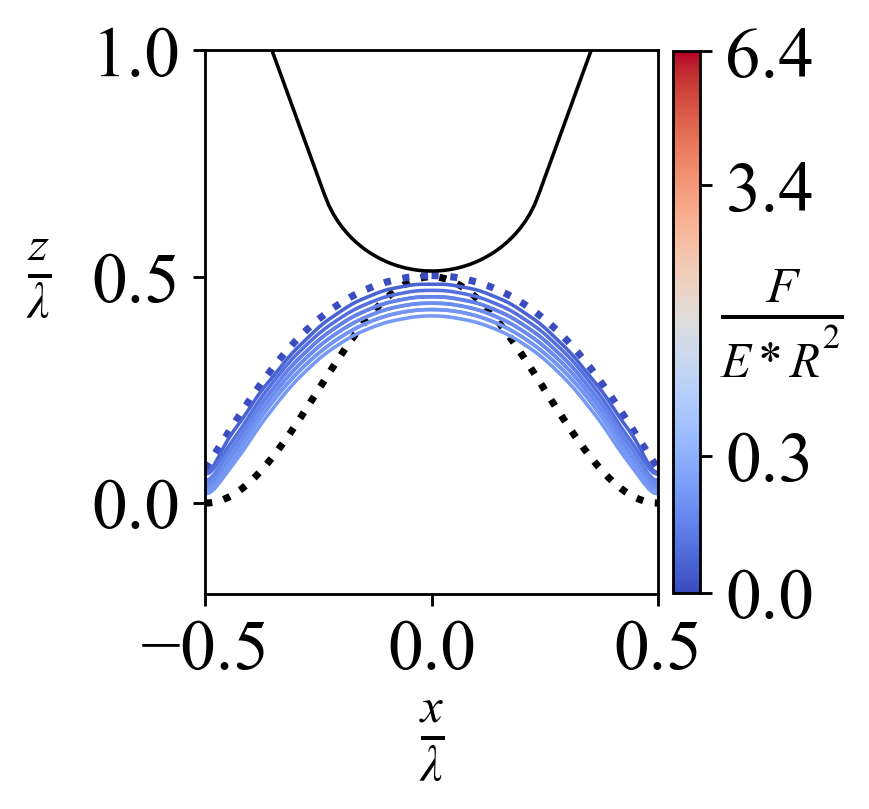
\includegraphics[width=1\linewidth]{Figures/Wave-LineContour-5.png}
    \end{subfigure}   
    % \hfill
    % \begin{subfigure}{0.32\textwidth}
    %     \centering
    %     \caption{\label{fig: All-Wave-FInterpolate-5}}
    %     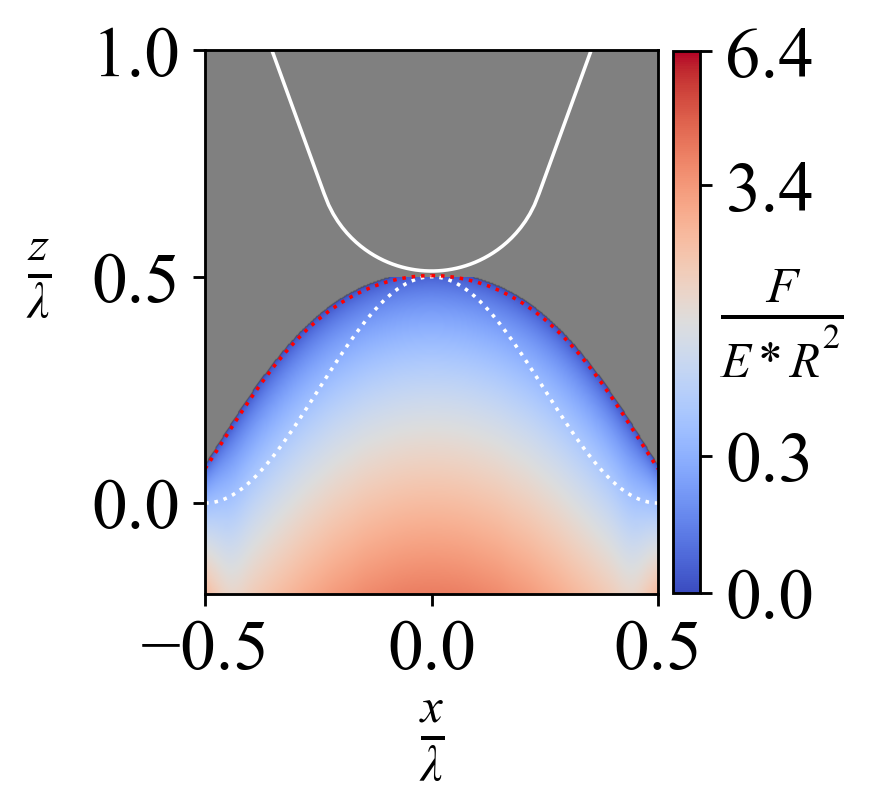
\includegraphics[width=1\linewidth]{Figures/Wave-FInterpolate-5.png}
    % \end{subfigure}   



    \hfill
    \vspace{-0.3in}
    
    
    
    \begin{subfigure}{0.32\textwidth}
        \centering
        \caption{\label{fig: All-Wave-ContourPlot-7}}
        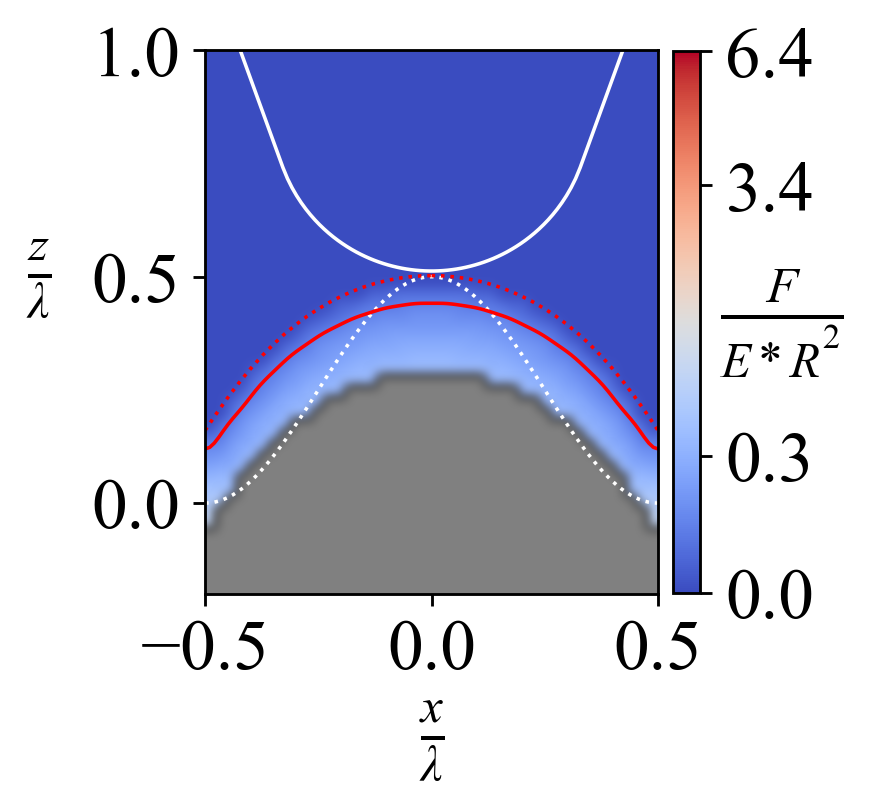
\includegraphics[width=1\linewidth]{Figures/Wave-ContourPlot-7.png}
    \end{subfigure}  
    \hfill  
    \begin{subfigure}{0.32\textwidth}
        \centering
        \caption{\label{fig: All-Wave-ContourPlotNI-7}}
        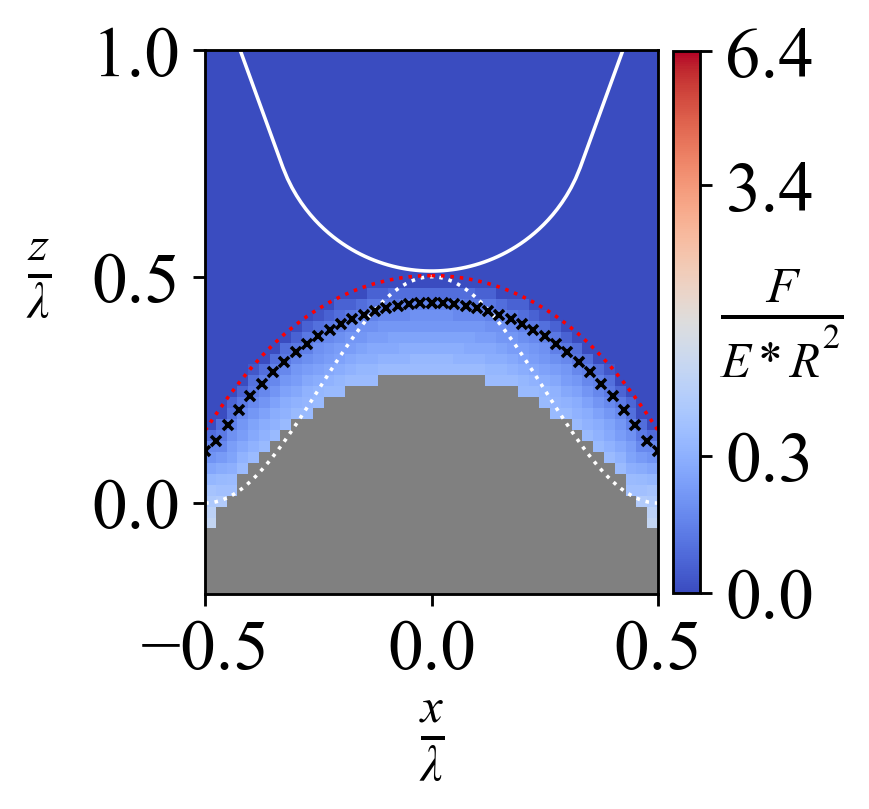
\includegraphics[width=1\linewidth]{Figures/Wave-ContourPlotNI-7.png}
    \end{subfigure}  
    \hfill  
    \begin{subfigure}{0.32\textwidth}
        \centering
        \caption{\label{fig: All-Wave-LineContour-7}}
        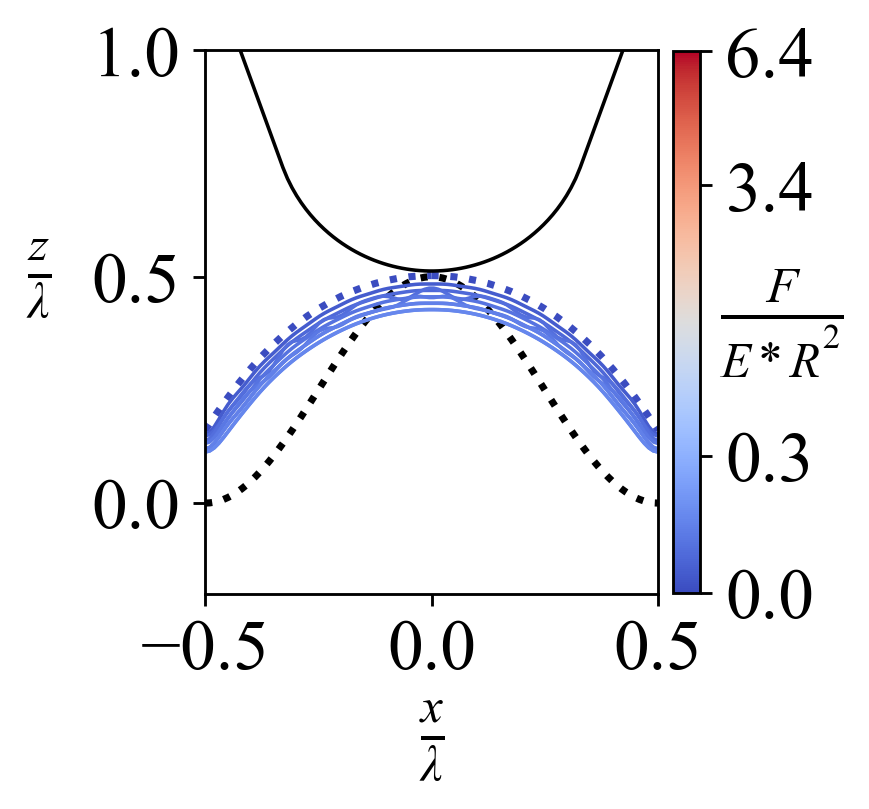
\includegraphics[width=1\linewidth]{Figures/Wave-LineContour-7.png}
    \end{subfigure}  
    % \hfill  
    % \begin{subfigure}{0.32\textwidth}
    %     \centering
    %     \caption{\label{fig: All-Wave-FInterpolate-7}}
    %     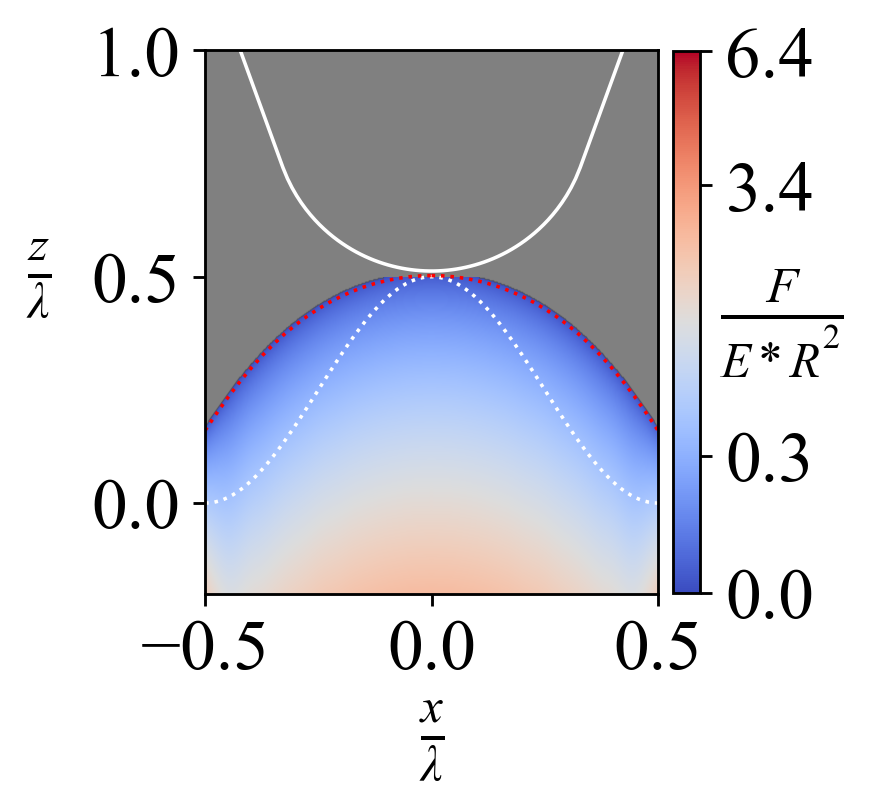
\includegraphics[width=1\linewidth]{Figures/Wave-FInterpolate-7.png}
    % \end{subfigure}  


    
    \hfill
    \vspace{-0.3in}
    

    
    \begin{subfigure}{0.32\textwidth}
        \centering
        \caption{\label{fig: All-Wave-ContourPlot-9}}
        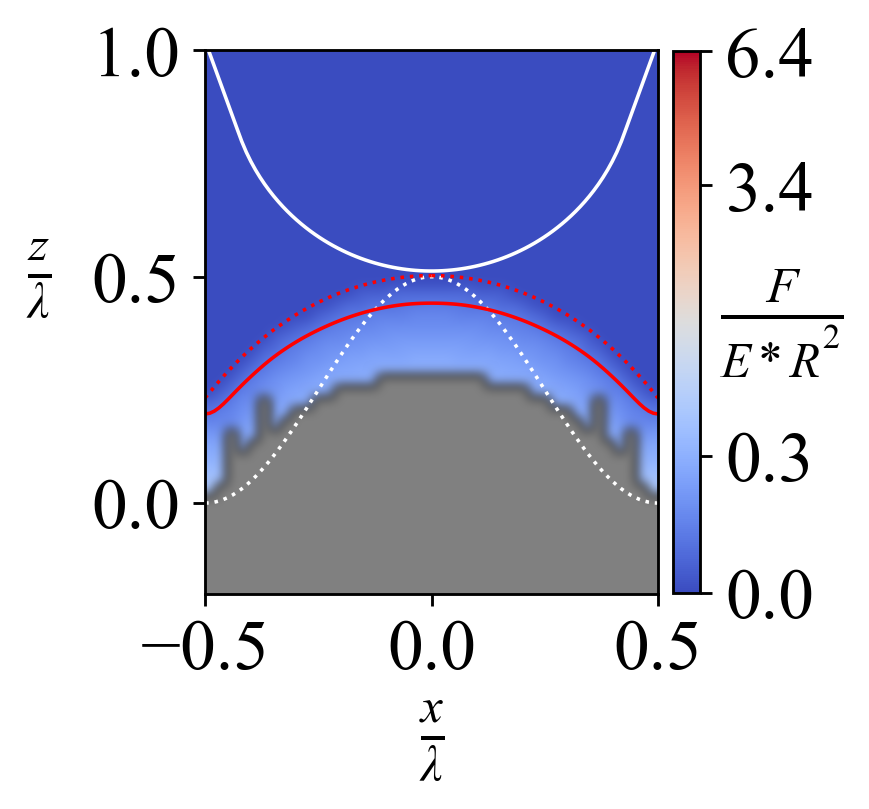
\includegraphics[width=1\linewidth]{Figures/Wave-ContourPlot-9.png}
    \end{subfigure}  
    \hfill
        \begin{subfigure}{0.32\textwidth}
        \centering
        \caption{\label{fig: All-Wave-ContourPlotNI-9}}
        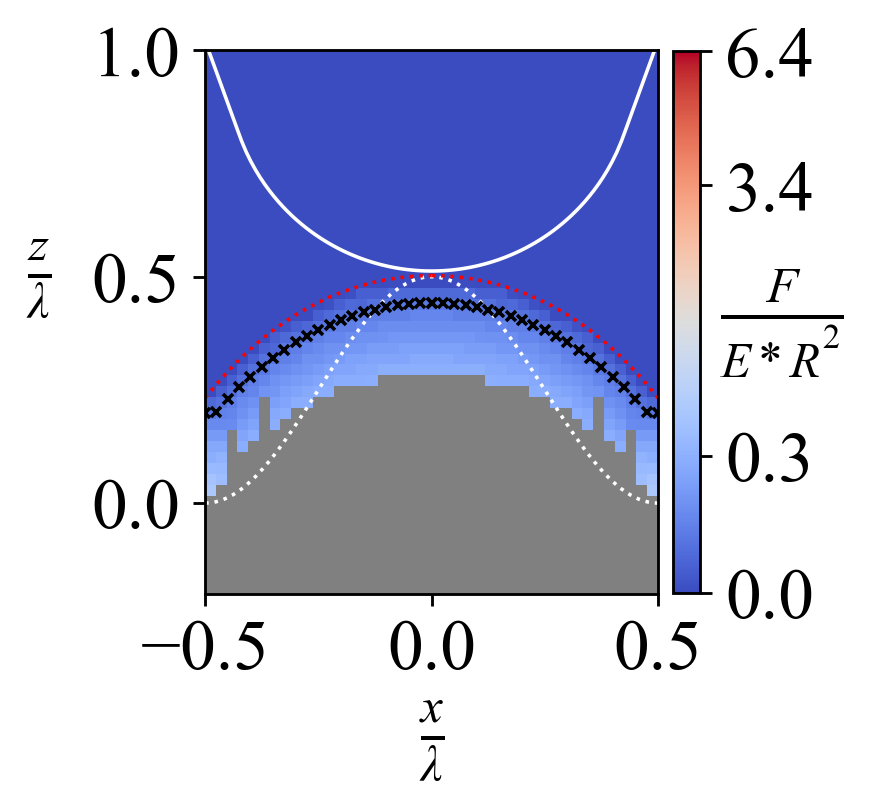
\includegraphics[width=1\linewidth]{Figures/Wave-ContourPlotNI-9.png}
    \end{subfigure}
    \hfill
    \begin{subfigure}{0.32\textwidth}
        \centering
        \caption{\label{fig: All-Wave-LineContour-9}}
        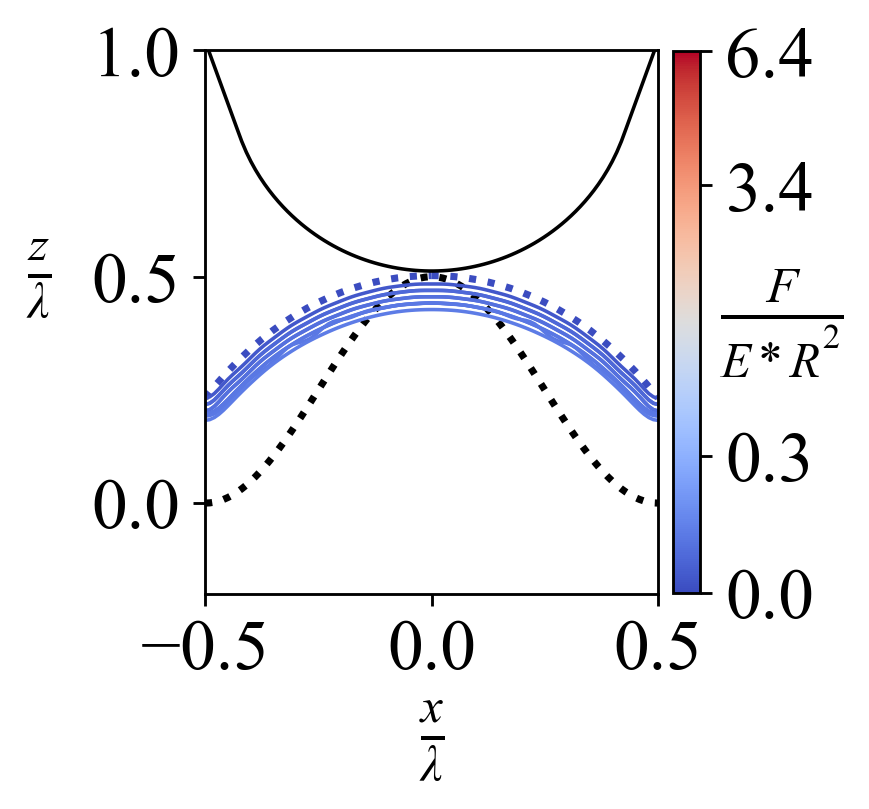
\includegraphics[width=1\linewidth]{Figures/Wave-LineContour-9.png}
    \end{subfigure} 
    % \hfill
    % \begin{subfigure}{0.32\textwidth}
    %     \centering
    %     \caption{\label{fig: All-Wave-FInterpolate-9}}
    %     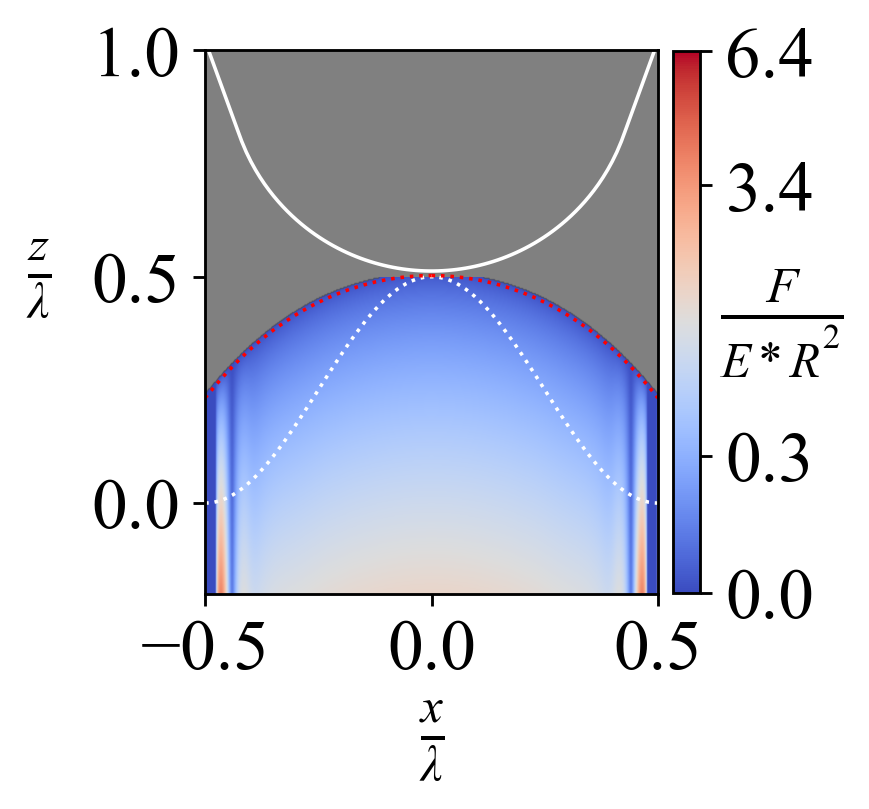
\includegraphics[width=1\linewidth]{Figures/Wave-FInterpolate-9.png}
    % \end{subfigure}

    \vspace{-0.3in}

    
    \caption{\label{fig: All-Wave-ContourPlot} }
\end{figure}